As previously mentioned, our goal is to design and develop a tool that will asssist the user in gathering insightful data from unorganized data.
In order to achieve this target we decided to implement various methods into our project.
Figure 1.1 displays the architecture designed for this system.
\begin {figure} [h]
    \centering
    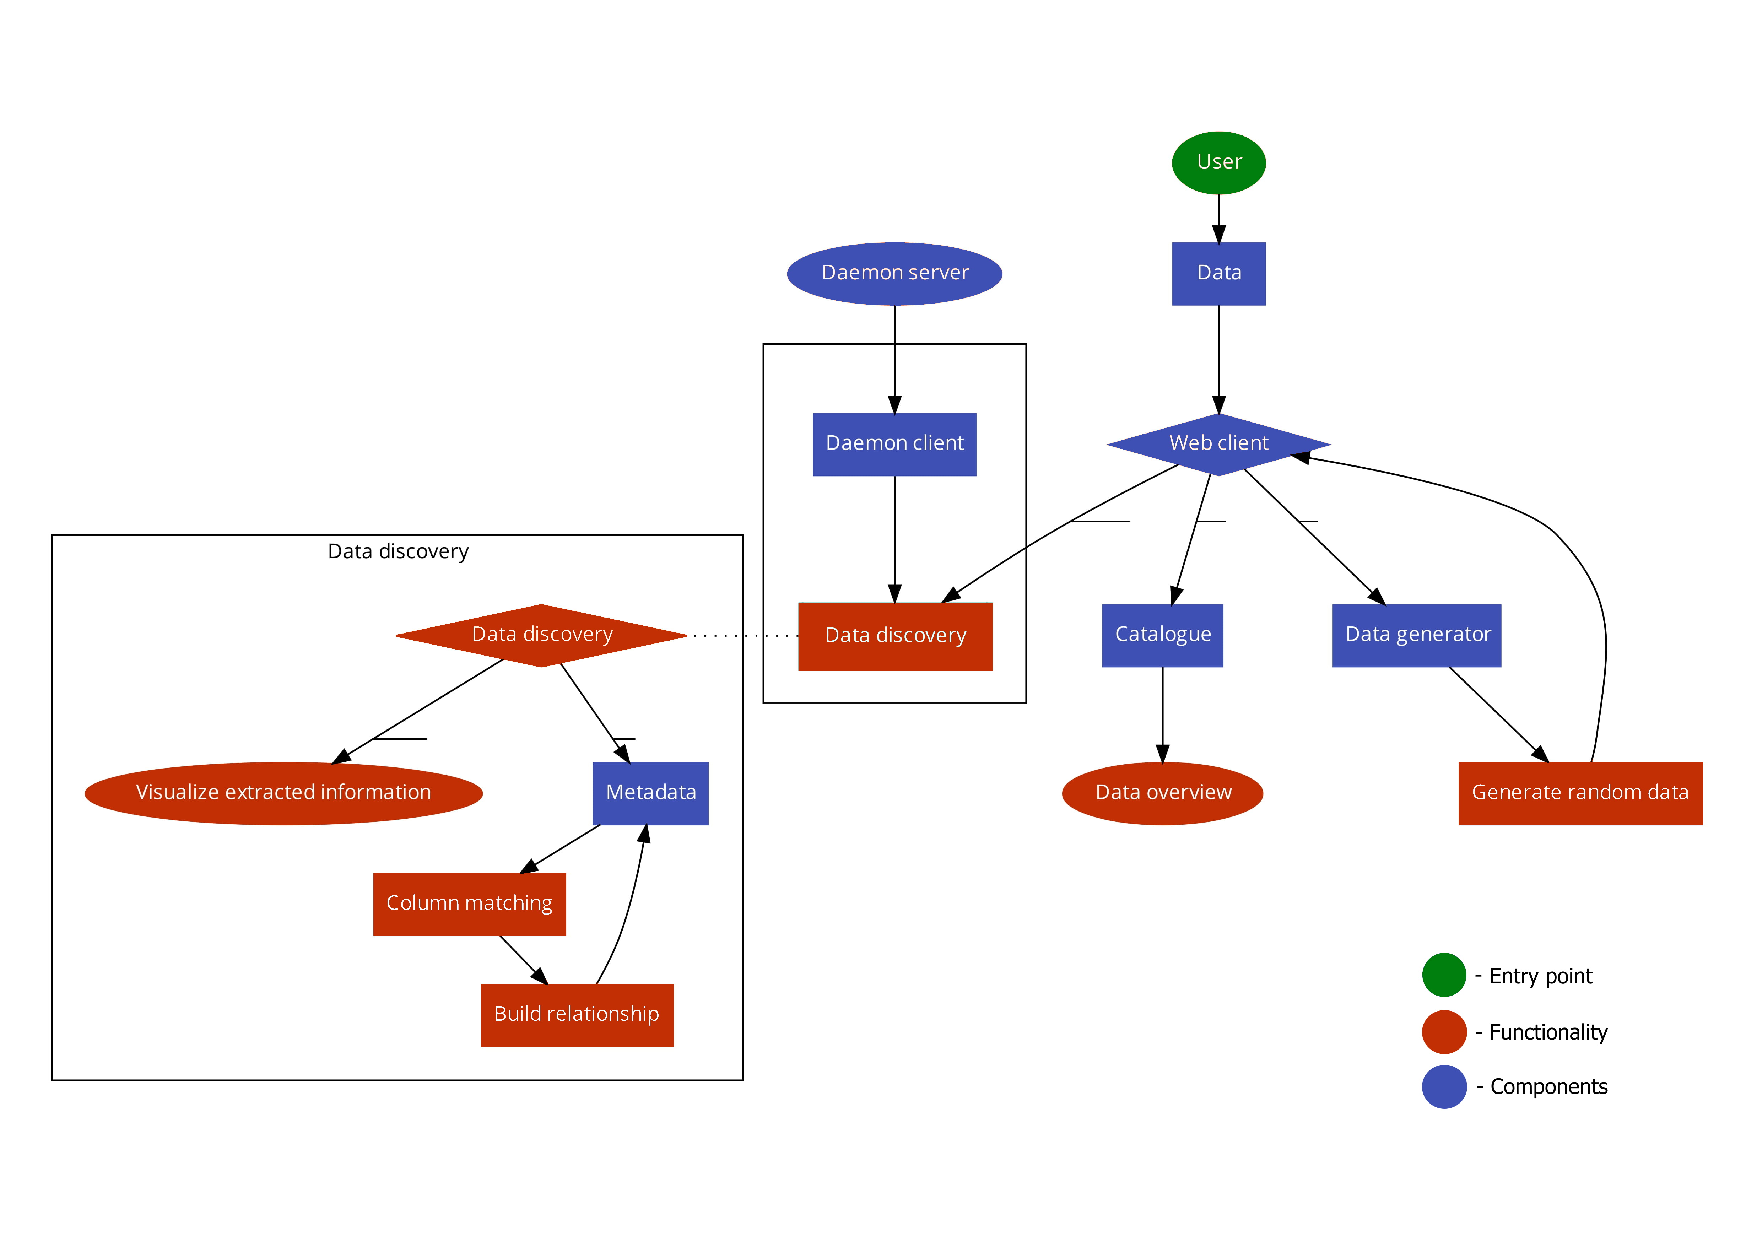
\includegraphics[width=16cm]{figures/architecture}
    \caption {Architecture of the data catalog \& data discovery system}
    \label {fig:architecture_diagram}
\end{figure}

To understand this diagram, we must focus on the core of the system, which consists of two key elements: the metadata and
the data matching library.
We consider these to be of critical importance, because the metadata is our chosen representation of information in the
catalog and the matching library is the primary building tool that gathers and structures this information.
Every other component has merely a supportive role.
We describe the metadata in detail in Section ~\ref{sec:metadata}, and the data matching library in Sections
~\ref{sec:discovery-strategy} and ~\ref{sec:the-data-matching-library}.

We present implementation details in Section ~\ref{sec:discovery-tool-implementation}, as a proof of concept of a system
that can reliably make use of the algorithms included in the library.
We include a web client in Section~\ref{sec:user-interface} that serves as both a management and display tool for the catalog.
For example, the web client is capable of requesting random data to be generated for testing.
Alternatively, for scenarios in which the user might need static reports instead of a full-blown web interface, we implemented
a metadata visualizer (Section~\ref{sec:metadata-visualization}).

The user interface can also be considered a use case of our product.
There are many others we came up with to showcase the various capabilities of our tool, all of them described in
Chapter~\ref{ch:applications}.
In our prototypes, we utilize two kinds of data.
First, there is the real world data.
The advantage of using this kind of data is that we can create a concrete demonstration of the tool's ability to solve problems
encountered by potential users.
The nature of these problems and how our data catalog might come in handy is explained in Section~\ref{sec:real-world-data}.
Then, there is generated data.
While modeled to reflect pattern that might be encountered in a real scenario, this data is clearly artificial (for example,
it can be just a sine wave), but it has the potential to test the performance of our system, by providing us easy access
to large amounts of it, without needing to access expensive sources.
We built our own random data generator, which we showcase in Section~\ref{sec:random-data-generator}.

In order to reach the goal of high system performance, we asked ourselves the question of why or when we would generate or
update metadata.
The answer is, whenever a new file enters the catalog or when an existing file changes.
Therefore, we need a way to check if a file was modified since the last metadata update and a component that can monitor
these changes.
The considerations behind checksum calculation can be found in Section~\ref{sec:checksum-calculation} and the file monitoring
daemon is explained in Section~\ref{sec:daemonized-file-monitoring}.
In testing of this part of the system, we are making heavy use of random data created by our generator.

With this design, we are aiming to achieve and demonstrate a number of key drivers behind a successful data catalog: scalability
(intensive performance testing and monitoring), usability (powerful user interface, variety of realistic use cases), and
innovation (the core of the system unlocks functionality that is not available in the existing solutions on the market).

\vspace{5mm} %5mm vertical space
\subsection{Catalogue}
The catalogue offers an overview of the respective data. Further on, the catalogue will allow the user to see all the column relationship created by the metadata. Additionally, the user can also make changes to his data as for example, hiding unwanted columns.
\vspace{5mm} %5mm vertical space
\subsection{Data generator}
For testing purposes, we decided to create our own random data generator. We ended up with this decision because we believe that this will enable us to mold the data as we would like. Our data generator creates a simple table, and each column can be either numerical or categorical. As the title suggested, the data generated is random and doesn't replicate real life data. In order to combat performance issues, our approach was to abstract each column into its own class in order to build an arbitrary dataframe
on the specified columns. This choice enabled us to generate a big amount of "fake" data that can be easily used to further develop our main tool. An example of this data generator can be found on the web client.
\vspace{5mm} %5mm vertical space
\subsection{Data Discovery}
The goal of data discovery is to analyze and extract insight from the the provided data. The information gathered will be later used by metadata to build potential relationship between the columns in order to provide the user with insightful and relevant information about his data. Further on we can use this information to represent it in a more organized way. Our approach for data discovery was to take two files and try to match columns between those two files using multiple techniques.

\vspace{5mm} %5mm vertical space
\subsection{Metadata}
Metadata is one of the main features of our data discovery tool. The main point of metadata is to use all the information delivered by data discovery in order to create relationship between columns and files. In short, metadata is data that describes data.
\newline
Some of the objectives for our metadata were that we wanted our metadata to generate human-readable information, but at the same time to also use a pre-existing format and have a low overhead. We also didn't want the users to be forced in installing a third party software in order to access the generated databases.
\newline

\clearpage
